\documentclass[a4paper, 12pt]{article}
\usepackage[T1]{fontenc}
\usepackage[scale=1,angle=0,opacity=1,color=black!60]{background}
\usepackage{tikzpagenodes}
\usepackage{lastpage}
\usepackage{lmodern}
\usepackage{float}
\usepackage{adjustbox}
\usepackage{amsmath}
\usepackage{nccmath}
\usepackage{url}
\usepackage{listings}
\usepackage{alltt}
\usepackage[section]{placeins}
\usepackage{tocloft}
\usepackage{hyperref}
\usepackage[textwidth=420pt,textheight=630pt]{geometry}
\usepackage[spanish, activeacute]{babel} %Definir idioma español
\usepackage[utf8]{inputenc} %Codificacion utf-8
\usepackage{listings}
\hypersetup{
    colorlinks,
    citecolor=black,
    filecolor=black,
    linkcolor=black,
    urlcolor=blue
}
\renewcommand{\cftsecleader}{\cftdotfill{\cftdotsep}}  % lineas punteadas en la tabla de contenidos
\setlength{\oddsidemargin}{15.5pt}
\backgroundsetup{contents={}} %Saca el 'draft'
\definecolor{mygray}{rgb}{0.95,0.95,0.95}
\lstset{
    basicstyle=\footnotesize,
    backgroundcolor=\color{mygray},         
    breaklines=true,
    breakatwhitespace=true,   
    postbreak=\mbox{\textcolor{red}{$\hookrightarrow$}\space},              
    captionpos=b,                    
    keepspaces=true,                 
    numbers=left,                    
    numbersep=5pt,                  
    showspaces=false,                
    showstringspaces=false,
    showtabs=false,
    tabsize=4,
    language=C,
    frame=none,
    title=\lstname,
}
\def\labelitemi{$\bullet$}

%\usepackage{titlesec}
\usepackage{hyperref}

\titleclass{\subsubsubsection}{straight}[\subsection]

\newcounter{subsubsubsection}[subsubsection]
\renewcommand\thesubsubsubsection{\thesubsubsection.\arabic{subsubsubsection}}
\renewcommand\theparagraph{\thesubsubsubsection.\arabic{paragraph}} % optional; useful if paragraphs are to be numbered

\titleformat{\subsubsubsection}
  {\normalfont\normalsize\bfseries}{\thesubsubsubsection}{1em}{}
\titlespacing*{\subsubsubsection}
{0pt}{3.25ex plus 1ex minus .2ex}{1.5ex plus .2ex}

\makeatletter
\renewcommand\paragraph{\@startsection{paragraph}{5}{\z@}%
  {3.25ex \@plus1ex \@minus.2ex}%
  {-1em}%
  {\normalfont\normalsize\bfseries}}
\renewcommand\subparagraph{\@startsection{subparagraph}{6}{\parindent}%
  {3.25ex \@plus1ex \@minus .2ex}%
  {-1em}%
  {\normalfont\normalsize\bfseries}}
\def\toclevel@subsubsubsection{4}
\def\toclevel@paragraph{5}
\def\toclevel@paragraph{6}
\def\l@subsubsubsection{\@dottedtocline{4}{7em}{4em}}
\def\l@paragraph{\@dottedtocline{5}{10em}{5em}}
\def\l@subparagraph{\@dottedtocline{6}{14em}{6em}}
\makeatother

\setcounter{secnumdepth}{4}
\setcounter{tocdepth}{4}


\begin{document}		
	% TÍTULO, AUTORES Y FECHA
	\begin{titlepage}
		\vspace*{\fill}
		\begin{center}
			\Large 75.43 Introducción a los sistemas distribuidos \\
			\Huge Entrega Trabajo Práctico 3: Enlace \\
			\bigskip\bigskip\bigskip
			\large\textbf{Integrantes:} \\
			\begin{center}
				\begin{tabular}{||c | c||} 
					\hline
					Alumno & padron \\ [0.5ex] 
					\hline\hline
					Azcona, Gabriela Mariel & 95363 \\
					\hline
					Avigliano, Patricio Andres & 98861 \\
					\hline
					Blanco, Sebastian Ezequiel & 98539 \\
					\hline
				\end{tabular}
			\end{center}
			\textbf{Fecha de Entrega:} 23/10/2018\\
			\textbf{GitHub:} https://github.com/BlancoSebastianEzequiel/Datacenter\\

		\end{center}
		\vspace*{\fill}
	\end{titlepage}
	\pagenumbering{arabic}
	\newpage
			
	% ÍNDICE
	\tableofcontents
	\newpage
	\pagenumbering{arabic}
	\section{Introducción teórica}
		\begin{itemize}
	\item \underline{\textbf{SDN:}}\\
		Software Defined Networking es un paradigma que puede considerarse reciente en el cual los dispositivos intermediarios 			encargados de conmutar paquetes son configurados por una entidad controladora por medio de software. Decimos dispositivos 			intermediarios porque este nuevo paradigma permite una configuración tan flexible que se pierde la distinción entre switches, 			routers, NATs; ahora cada dispositivo se configura según las necesidades particulares de la red en la que habita.

	\item \underline{\textbf{OpenFlow:}}\\
		Es la herramienta que se utiliza para implementar esta nueva tecnología, mejor dicho es el protocolo por el cual se configuran 			los dispositivos intermediarios. La idea principal es reemplazar las tablas de ruteo de los routers y las tablas de direcciones 		Mac en los switches por tablas de flujo. Entonces un dispositivo OpenFlow decide qué hacer con los paquetes que le llegan en 			base a la tabla de flujo, por otro lado se configuran las políticas y el comportamiento que debe adoptar mediante el protocolo 			OpenFlow.

	\item \underline{\textbf{Control y Forwarding path:}}\\
		Un dispositivo de internet por definición debe funcionar con la mayor velocidad posible, por ello su funcionamiento está 			implementado por hardware y el costo de implementarlo exclusivamente por software en cuanto a velocidad sería muy elevado. Es 			por eso que los dispositivos OpenFlow se dividen en 2 planos: el plano de datos o forwarding (hardware) y el plano de control 			(software), este último es el que se comunica por medio de OpenFlow con la entidad controladora que indicará cómo deberá ser 			administrado el dispositivo. El plano de datos hará lo que sea necesario con cada paquete según la tabla de flujos mientras que 		el plano de control gestionará las decisiones a tomar sobre la construcción de la tabla, modificación de algún parámetro de la 			cabecera (por ejemplo al implementar Network Address Translation) y políticas de seguridad, entre otras funcionalidades.

	\item \underline{\textbf{Concepto de flujo:}}\\
		No existe una definición per se de lo que es un flujo pero lo entendemos como el conjunto de paquetes que esperamos que llegue 			de un mismo origen a un mismo destino (por destino y origen nos referimos a nivel enlace/red/transporte) con similar latencia y 		por el mismo camino. Un ejemplo podría ser la respuesta de un http get, todos los paquetes de la respuesta provienen del mismo 			origen, van hacia el mismo destino y se espera que lleguen medianamente uno detrás del otro (suponiendo no haya pérdidas). Para 		lo que es un dispositivo OpenFlow un flujo se define como la 10-tupla formada por (PortIn, VLANID, srcEth, dstEth, typeEth, 			srcIP, dstIP, protoIP, srcport, dstport) y es sobre estos campos que se definen las entradas en la tabla de flujos, luego 			podrán utilizarse los campos que sean necesarios según las políticas adoptadas por el plano de control.

	\item \underline{\textbf{IP blackholing:}}\\
		Es la decisión que se toma de descartar paquetes provenientes de una determinada dirección IP al detectar un ataque, los 			dispositivos OpenFlow permiten introducir políticas sobre lo que debe ser considerado como un ataque y en qué casos hacer IP 			blackholing de manera flexible y que se adapte a la sensibilidad de la red en la que está funcionando.

	\item \underline{\textbf{Firewall:}}\\
		Es un mecanismo de seguridad cuya función es proteger la red interna frente amenazas de redes no confiables, para ello puede 			filtrar o redireccionar los paquetes que se consideran como no permitidos según ciertas reglas de seguridad. Por ejemplo si no 			queremos contestar paquetes ICMP podemos configurar para que todos los paquetes de ese protocolo sean descartados. Devuelta lo 			que permite OpenFlow es adaptar el firewall del dispositivo según las necesidades particulares de la red.
\end{itemize}


		\begin{figure}[ht]
			\begin{adjustbox}{addcode={
				\begin{minipage}{\width}}{
					\caption{%
						Ejemplo de como seria la topologia con un arbol de altura 3.
						}
				\end{minipage}},rotate=360,center}
				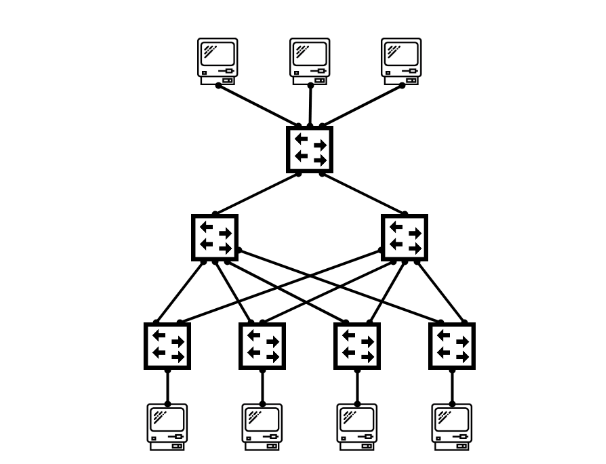
\includegraphics[scale=.6]{pics/topologia-arbol-altura-3.png}
			\end{adjustbox}
		\end{figure}
		\FloatBarrier
	\newpage
	\section{Objetivo}
		La idea del trabajo es familiarizarse con la tecnología de las SDNs y el protocolo OpenFlow, junto con las diversas problemáticas que permiten enfrentar; como objetivo secundario veremos una arquitectura de datacenters. Para ello simularemos mediante Mininet la estructura de un datacenter pequeño conectado bajo la topología Fat-Tree y configuraremos los switches mediante OpenFlow


	\newpage
	\section{Desarrollo}
		\subsection{Preguntas}	
	\begin{enumerate}
		\item ¿Cuál es la diferencia entre un Switch y un router? ¿Qué tienen en común?
			\underline{\textbf{Diferencias:}}
				\begin{itemize}
					\item Direccionamiento dentro de la misma red
					\item Confección de la tabla de ruteo
						\begin{itemize}
							\item Los switches aprenden a partir de la direccion origen
							\item Los routers aprenden a partir de la direccion destino
						\end{itemize}
					\item Metodología de ruteo (broadcast en SW)
					\item Configuración (plug-n-play vs DFGW)
					\item El router es el dispositivo que se encarga de reenviar los paquetes entre distintas redes
					\item El router es mas  ``inteligente`` que el switch, ya que además de cumplir con la misma función, 						tiene además la capacidad de escoger la mejor ruta para que un determinado paquete de datos llegue a su 					destino
					\item Los routers son capaces de interconectar varias redes y generalmente trabajan en conjunto con 						hubs y switchs.
				\end{itemize}
			\underline{\textbf{Similitudes:}}
				\begin{itemize}
					\item Ambos envían información en elementos discretos (tramas vs datagramas)
					\item Ambos tienen una tabla para decidir como enviar los paquetes
				\end{itemize}
		\item ¿Cuál es la diferencia entre un Switch convencional y un Switch OpenFlow?\\
			Un switch normal funciona independientemente del resto de la red.

			Un switch OpenFlow, cuando recibe un paquete, para el cual no tiene un flujo de salida, es decir, que en la tabla del 				switch no tiene un match respecto de la direccion de entrada, se pondrá en contacto con un controlador y le preguntará 				qué debe hacer con este paquete. Luego, el controlador puede actualizar la tabla del switch, posiblemente incluyendo 				alguna manipulación de paquetes. Una vez que el flujo se descarga al conmutador, cambiará los paquetes similares a 				velocidad de cable.
		\item ¿Se pueden reemplazar todos los routers de la Intenet por Swithces OpenFlow?(Piense en el escenario interASes para 			elaborar su respuesta)\\
			Si pensamos en router normales se podrian cambiar facilmente, pero habria que tener en cuenta que debe haber varios 				controladores, porque si todos acceden al mismo, este mismo colapsaria y no podria atender a todos los pedidos al mismo 			tiempo (siedo que estamos remplazando muchos router de toda la internet). \\
			Si pensamos en los sistemas autonomos, tenemos los routers de borde que tiene una caracteristica en particular, y esta 				es que manejan un protocolo llamado BGP en donde se puede decidir que prefijos se dan a conocer, se elijen los 				protocolos de ruteo, se determina la ingenieria de trafico y demas caracteristicas. Por lo tanto habria que tener un 				controlador especial para estos donde se pueda manejar la logica del mismo y que ademas sean configurables ya que 				sabemos que la discrecionalidad de los prefijos se da por acuerdo comerciales, entonces, frente a cambios en estos 				acuerdos, se debe poder cambiar dicha discrecionalidad de una manera efectiva en el controlador de manera tal que sea 				flexible frente a cambios. Esto haria que sea mas facil la configuracion.
	\end{enumerate}

\subsection{Maquina virtual}
	Necesitamos de la maquina virtual (VM) para poder ejecutar el controlador, el firewall y la topologia. Por lo tanto debemos usar 		distintas terminales de la misma para ello. Hay dos formas de hacer esto: una es usar la interfaz que provee la VM y abrir terminales 		desde alli. La otra es abrir terminales desde nuestra pc, y conectarnos via ssh a la maquina virtual. Parece que la primera opcion es 		mas comoda, pero en mi experiencia la VM se traba mucho mas.
	Para conectarse via ssh a la VM, primero clonamos nuestro repositorio y solo necesitamos ejecutar un script que hace el trabajo.
	\begin{lstlisting}[language=bash,numbers=none]
	 	$ sh scripts/conect_to_VM.sh
	\end{lstlisting}	
	Nos pedira la cotraseña de nuetra pc, y luego la contraseña de la VM que es: \lstinline[columns=fixed]{frenetic}.\\
	Luego, si queremos tener nuestro repositorio en la VM, y ademas el controlador en la carpeta \lstinline[columns=fixed]{pox/ext/} del 		repositorio de pox en la VM, debemos ejecutar el siguiente comando:\\
	\begin{lstlisting}[language=bash,numbers=none]
		$ sh scripts/resync.sh
	\end{lstlisting}
\subsection{Topologia}
	La topologia que se desarrollo se llama Fat tree. En la siguiente figura vemos nuetra topologia por defecto que es un árbol de altura 3.
	La raiz tiene conectada 3 hosts que funcionan como clientes del datacenter, cada una de las raices a su vez, tendrán conectadas un host 	cada una, que funcionará como proveedor de contenido.\\
	Los tres hosts clientes se comunican con los hosts del datacenter usando los protocolos ICMP, TCP y UDP.
	\begin{figure}[ht]
		\begin{adjustbox}{addcode={
			\begin{minipage}{\width}}{
				\caption{%
					Ejemplo de como seria la topologia con un arbol de altura 3.
					}
			\end{minipage}},rotate=360,center}
			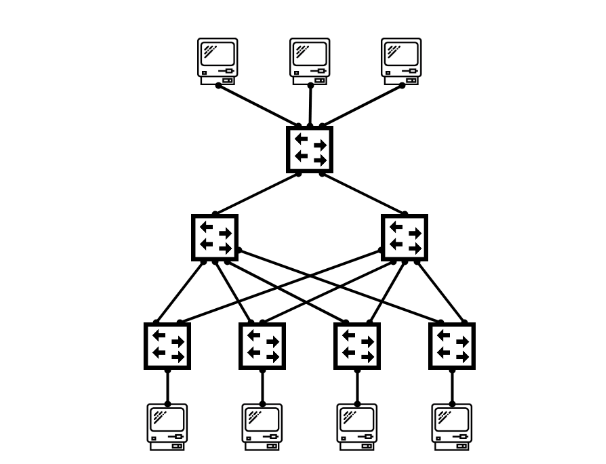
\includegraphics[scale=.6]{pics/topologia-arbol-altura-3.png}
		\end{adjustbox}
	\end{figure}
	\FloatBarrier
	Para poder levantar la topologia sin pasarle los argumentos de configuracion, lo cual hace que por defecto tenga tres clientes y una 		altura de tres, abrimos una terminal que este en la raiz del sistema de archivos de la maquina virtual y podemos escribir 
	lo siguiente:\\
	\begin{lstlisting}[language=bash,numbers=none]
		sudo mn --custom ~/Datacenter/src/topology.py --topo mytopo --mac --switch ovsk --controller remote
	\end{lstlisting}
	En caso de querer configurar la altura o cantidad de clientes, podemos escribir lo siguiente:\\
	\begin{lstlisting}[language=bash,numbers=none]
		sudo mn --custom ~/Datacenter/src/topology.py --topo mytopo, levels=4, clients=4 --mac --switch ovsk --controller remote
	\end{lstlisting}
	
	Hay una heramienta para visualizar topologias a partir de nuestra salida en mininet. Si en mininet escribimos el comando 
	\lstinline[columns=fixed]{dump} y el comando \lstinline[columns=fixed]{links} podemos usar cada salida en una pagina de internet, que 		el link esta en la referencias, la cual se pega cada salida como se explica en dicha pagina y nos genera un arbol. De esta manera 		podemos comprobar que nuestra topologia se creo correctamente como se ve a continuacion:\\
	\begin{figure}[ht]
		\begin{adjustbox}{addcode={
			\begin{minipage}{\width}}{
				\caption{%
					Topologia generada con los comandos dump y links de mininet.
					}
			\end{minipage}},rotate=360,center}
			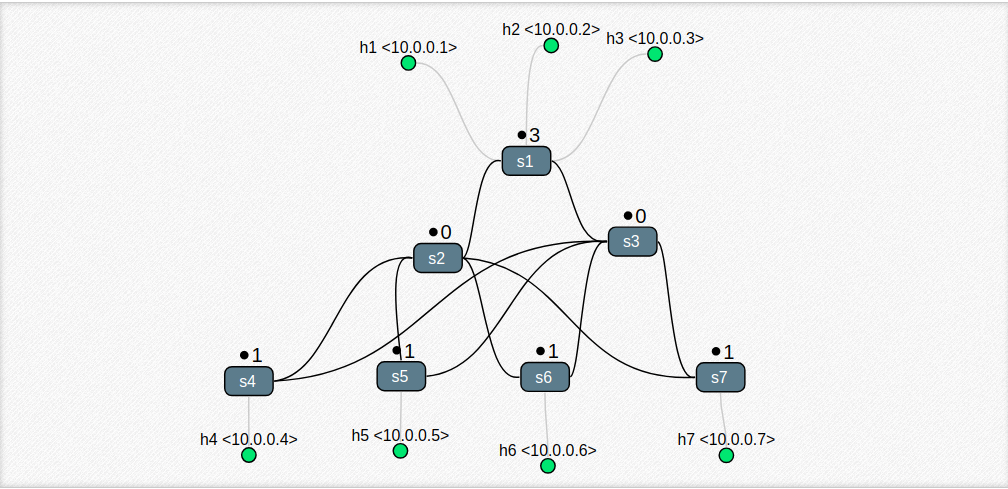
\includegraphics[scale=.6]{pics/dump_link_topo.png}
		\end{adjustbox}
	\end{figure}
	\FloatBarrier

\subsection{Controlador}
	El controlador se encarga de la logica del balanceo de cargas y tambien se encarga de llenar las tablas de los switch cuando estos les 		llega un mensaje que no saben responder. De esta manera nuestro controlador consta de \lstinline[columns=fixed]{handlers} los cuales se 	ejecutan cuando un switch acude al controlador.\\
	El controlador hace un estudio de la topologia para poder obtener un diccionario de adyacencias, el cual sera util para poder calcular 		el camino minimo para el balanceo de cargas.\\
	\underline{\textbf{\_handle\_LinkEvent:}}\\
		Este handler es invocado cada vez que se detecta un link entre switches. El modulo \lstinline[columns=fixed]{Discovery} es el 			que se encarga de esto. Se envian mensajes LLDP entre los switches y de esta manera se puede aprender la topologia. En nuestro 			handler, cuando es invocado, llenamos un diccionario con la informacion pertinente.\\
	\underline{\textbf{host\_tracker:}}\\
		Es una clase de python que se encuentra en el repositorio de pox. En nuestro caso la utilizamos para poder descubrir el 		identificador del switch destino a partir de la direccion mac destino. Esto lo necesitamos porque las adyacencias se manejan 			con los identificadores de los switchs (dpid). Por eso, en el constructor del controlador se instancia el mismo, y por cada vez 		que se entra al handler que se encarga de llenar la tabla de los switches (\lstinline[columns=fixed]{_handle_PacketIn}), se 			llama al handler del \lstinline[columns=fixed]{host_tracker}, que se encarga de aprender los dpid. Luego, podremos obtener el 			identificador utilizando un metodo del \lstinline[columns=fixed]{host_tracker} el cual accede a un diccionario de entradas de 			direcciones mac, y retorna el dpid. Ese metodo es \lstinline[columns=fixed]{host_tracker.getMacEntry(addr)}\\
	\underline{\textbf{spanning tree:}}\\
		Este modulo se encarga de eliminar los ciclos de la topologia. Su función es la de gestionar la presencia de bucles en 			topologías de red debido a la existencia de enlaces redundantes. El protocolo permite a los dispositivos de interconexión 			activar o desactivar automáticamente los enlaces de conexión, de forma que se garantice la eliminación de bucles.\\
	\underline{\textbf{\_handle\_PacketIn:}}\\
		Este handler se invoca frente a la llegada de un paquete, cuando un switch no sabe como responder frente a el, es decir, la 			tabla del switch no tiene un match para despacharlo por un puerto y por lo tanto le pide ayuda al controlador. El algoritmo 			es bastante simple y consta de los siguientes pasos:
		\begin{itemize}
			\item Se llama al handler del \lstinline[columns=fixed]{host_tracker} para que aprenda los dpid de cada mac.
			\item Si el protocolo no es ni ICMP, o TCP o UDP se retorna
			\item Si el paquete es IPv6 se retorna
			\item Si el paquete ethernet no se encuentra, se retorna
			\item Si el paquete no es ni IP ni ARP, se retorna.
			\item Si la direccion mac destino, no se encuantra en nuestra tabla de matcheo de mac con dpid (generada a partir de la 			respuesta del \lstinline[columns=fixed]{host_tracker} al invocar 
			\lstinline[columns=fixed]{host_tracker.getMacEntry(addr)}, se hace flooding y retorna
			\item Si el dpid origen coindide con el destino, no hacemos nada y guardamos esto en la tabla.
			\item si son distintos:
			\begin{itemize}
				\item Se buscan todos los caminos minimos desde el dpid origen al destino en el diccionario de adyacencias.
				\item Si no hay caminos, se retorna
				\item si, existen caminos, se extrae de ellos los puertos de los cuales se sale del switch (seria el puerto de 					salida)
				\item Se actualiza la tabla del switch
				\item se envia el mensaje.
			\end{itemize}
		\end{itemize}
	\underline{\textbf{Tecnica ECMP - Balanceo de cargas:}}\\
		Para resolverlo se creo una clase en python llamada \lstinline[columns=fixed]{ECMPTable} la cual encapsula un diccionario que 			tiene como clave el identificador del switch corresponiente ($dpid$). Como valor de este identificador tiene otro diccionario 			en el cual su clave es una tupla de valores los cuales son, el identificador del switch destino ($dst\_dpid$), la direccion mac 		origen ($src\_addr$), la direccion mac destino ($dst\_addr$), y un string que nos dice el protocolo ($protocol$: [ICMP, TCP, 			UDP]). Como valor a esta clave se encuentra el puerto de salida. De esta manera, frente a distintos caminos de igual peso, 			dependiendo el flujo, los puertos de salida son distintos.

\subsection{Firewall}
	Se creo una clase llamada Firewall la cual, frente a la llegada de paquetes UDP, en caso de superar cierto maximo (en nuestro caso 		100), se los bloquea. Luego de un tiempo, se los desbloquea. Para poder llevarlo a cabo, se creo un metodo 
	llamado	$request\_for\_switch\_statistics$, el cual se llama cada un tiempo determinado mediante un timer. Este se encarga de pedirle 		las estadisticas a los switches, para poder calcular la frecuencia de paquetes UDP. Luego, tenemos otro handler 
	llamado $\_handle\_flowstats\_received$ el cual se llama cada vez que los witches nos proveen sus estadisticas. El algoritmos se 		pregunta que los paquetes tengan el protocolo UDP, y almacena su cantidad en un diccioanrio. En caso de que la diferencia de cantidades 	entre la vez actual y la anterior acumulada sea mayor que nuestro maximo propuesto, se procede a bloquear el paquete y se setea un 		timer para este. En caso de no superar est maximo, se chequea si ya se esta bloqueado, y en ese caso se chequea el paso del tiempo con 		los timers.

\subsection{Launch}
	Para poder levantar el controlador y el firewall, se creo un archivo llamado $launch.py$ que configura el spanning tree, el discovery, 		el controlador y el firewall.








	\newpage
	\section{Pruebas realizadas}
		\subsection{Configuracion}
	Para poder correr el controlador y la topologia debemos abrir la maquina virtual. Luego abrir dos terminales como se explico en la 		seccion de maquina virual en desarrollo. Pra resumirlo en pasos, debemos:
	\begin{enumerate}
		\item Pararse en la raiz del repositorio
		\item abrir una terminal y ejecutar: \lstinline[columns=fixed]{sh scripts/resync.sh} y cerra terminal
		\item Luego, abrir una terminal ejecutar: \lstinline[columns=fixed]{sh scripts/conect_to_VM.sh}. Nos pedira nuestra 			contraseña y la contraseña de la VM que es: \lstinline[columns=fixed]{frenetic}
		\item Correr el controlador ejecutando: \lstinline[columns=fixed]{pox/pox.py launch}
		\item Repetir el paso 3 en otra terminal.
		\item Levantar la topologia ejecutando: \lstinline[columns=fixed]{sh Datacenter/scripts/lift_topology.sh}
	\end{enumerate} 
\subsection{Pingall}
	Una vez que levantamos primero el controlador y luego la topologia, los sitches tienen su tabla vacia, por lo que el primer pingall 		sera consultado compeltamente al controlador para que resuelva las salidas. Por lo tanto el primer pingall siempre tardara un poco mas, 	y en algunos caso, algun ping puede llegar a perderse por un timeout. A continuacion mostramos un pingall apenas se levanto 
	la topologia y el controlador y otro pingall justo despues asi contrarestamos el tiempo que tardo cada uno:
	\begin{figure}[ht]
		\begin{adjustbox}{addcode={
			\begin{minipage}{\width}}{
				\caption{%
					Pingall apenas se levanto el controlador y la topologia
					}
			\end{minipage}},rotate=360,center}
			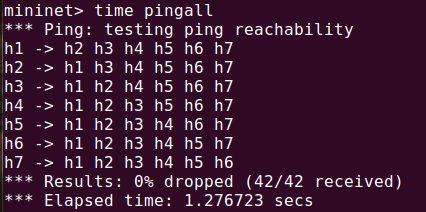
\includegraphics[scale=.6]{pics/pingall_1.png}
		\end{adjustbox}
	\end{figure}
	\FloatBarrier
	\begin{figure}[ht]
		\begin{adjustbox}{addcode={
			\begin{minipage}{\width}}{
				\caption{%
					Segundo Pingall
					}
			\end{minipage}},rotate=360,center}
			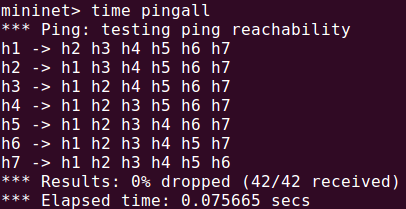
\includegraphics[scale=.6]{pics/pingall_2.png}
		\end{adjustbox}
	\end{figure}
	\FloatBarrier
	Podemos observar que no hubo perdidas, y ademas se ve claramente la diferencia de tiempo en que se resolvio los pings en cada caso 		donde en el primer caso se tardo unos $1.276723 \; segundos$ y en el segundo caso el tiempo disminuyo drasticamente 
	a unos $0.075665 \; segundos$.
\subsection{Balanceo de cargas con conexion TCP}
	Para realizar esta prueba vamos a utilizar la herrmienta $iperf$ para hacer una conexxion cliente-servidor entre dos hosts. Primero, 		vamos a ir a la terminal donde esta correindo mininet (donde levatamos la topologia) y en el prompt de mininet escribiremos 
	$xterm h1 h4$ para abrir dos terminales en cada host.\\
	Luego vamos a abrir otra terminal (conectada a la VM como se exlico antes) y escribiremos: $sudo \; wireshark \; \&$. Y abriremos la 		interfaz $s2-eth1$. Y abriremos otro wireshark de la misma manera, pero en la interfaz $s3-eth1$.\\
	Luego en la terminal del host 4 levantaremos el servidor escribriendo lo siguiente: 
	\begin{lstlisting}[language=bash,numbers=none]
		$ iperf -s -p 80
	\end{lstlisting}	
	En la terminal del host 1 escribiremos lo sigueinte para hacer la conexion: 
	\begin{lstlisting}[language=bash,numbers=none]
		$ iperf -c 10.0.0.4 -p 80
	\end{lstlisting} 
	Y lo que haremos es ver ambas ventanas de wireshark y comprobar que los paquetes TCP solo pasan por algunas de las dos interfaz, pero 		no en ambas.\\
	A continuacion mostramos la captura de las terminales en cada host. y la comprobacion del balanceo de cargas en wireshark:\\
	\begin{figure}[ht]
		\begin{adjustbox}{addcode={
			\begin{minipage}{\width}}{
				\caption{%
					Conexion TCP cliente host 1
					}
			\end{minipage}},rotate=360,center}
			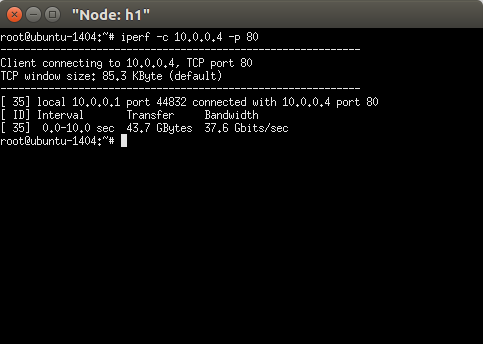
\includegraphics[scale=.6]{pics/iperf-h1-tcp.png}
		\end{adjustbox}
	\end{figure}
	\FloatBarrier
	\begin{figure}[ht]
		\begin{adjustbox}{addcode={
			\begin{minipage}{\width}}{
				\caption{%
					Conexion TCP servidor host 4
					}
			\end{minipage}},rotate=360,center}
			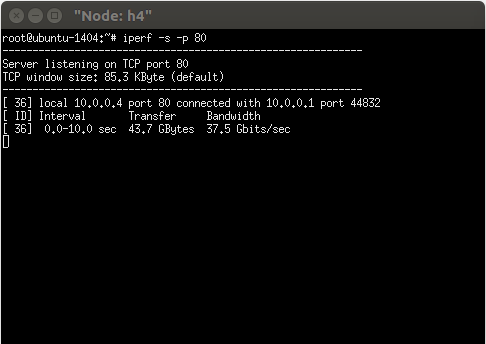
\includegraphics[scale=.6]{pics/iperf-h4-tcp.png}
		\end{adjustbox}
	\end{figure}
	\FloatBarrier
	Podemos comprobar que cumple con el balanceo de cargas ya que los paquetes solo viajan por el switch 2. Esto es asi, porque ir por 		cualquiera de los swtich es lo mismo respecto a llegar a desrino y a cuanto pesa el mismo, es decir, tenemos un empate y vemos que el 		controlador decidio que de acuerdo a este flujo se elija solo el switch 2:\\
	\begin{figure}[ht]
		\begin{adjustbox}{addcode={
			\begin{minipage}{\width}}{
				\caption{%
					Captura de wireshark monitoreando la interfaz eth1 del switch s2
					}
			\end{minipage}},rotate=360,center}
			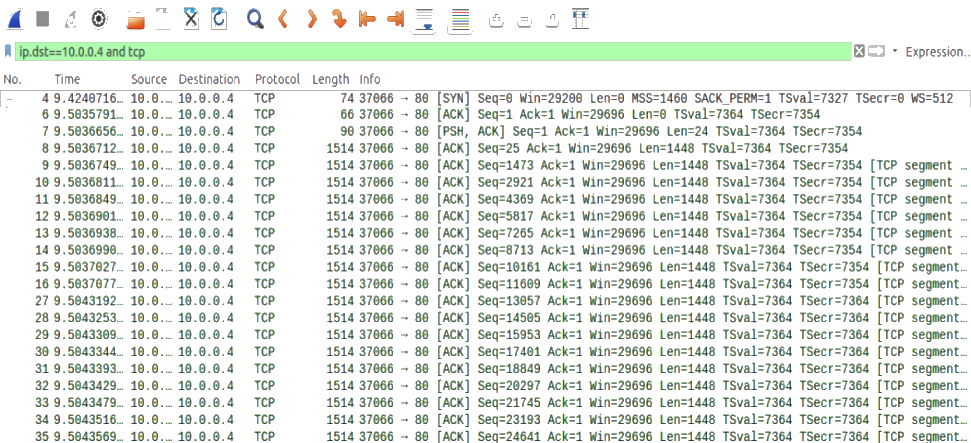
\includegraphics[scale=.6]{pics/s2-eth1-tcp-h1-h4.png}
		\end{adjustbox}
	\end{figure}
	\FloatBarrier
	\begin{figure}[ht]
		\begin{adjustbox}{addcode={
			\begin{minipage}{\width}}{
				\caption{%
					Captura de wireshark monitoreando la interfaz eth1 del switch s3
					}
			\end{minipage}},rotate=360,center}
			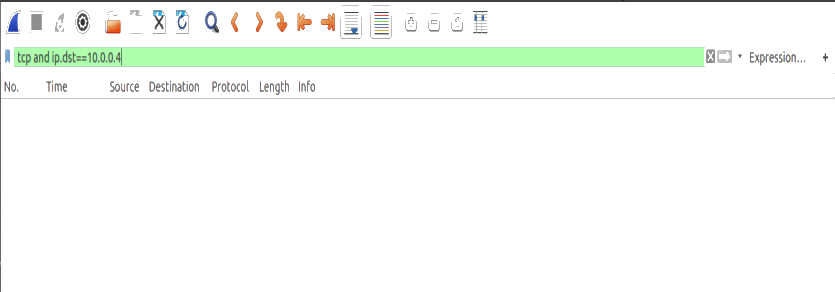
\includegraphics[scale=.6]{pics/s3-eth1-tcp-h1-h4.png}
		\end{adjustbox}
	\end{figure}
	\FloatBarrier

\subsection{Balanceo de cargas con ping}
	Para realizar esta prueba vamos a usar miniet haciendo un ping entre h1 y h5, y otro ping entre h2 y h5. De esta manera podremos ver 		que lo que deberia pasar es que un flujo deberia elegir el switch 2 o 3 y el otro flujo tambien sin que ambos elijan el mismo flujo. 		Los paquetes que se envian contienen un protocolo ICMP, por lo tanto haremos un monitoreo en la interfaces s3-eth1 y s2-eth1 para 		verificar que cuando hacemos el ping ehtre h1 y h5 una de ellas esta vacia y la otra recibe los paquetes, pero al hacer el ping entre 		h2 y h5 debemos poder ver los mismo pero en los switches invertidos.\\
	Primero mostramos el monitoreo en wireshark cuando hacemos el ping entre h1 y h5:\\
	\begin{figure}[ht]
		\begin{adjustbox}{addcode={
			\begin{minipage}{\width}}{
				\caption{%
					Captura de wireshark monitoreando la interfaz eth1 del switch s2
					}
			\end{minipage}},rotate=360,center}
			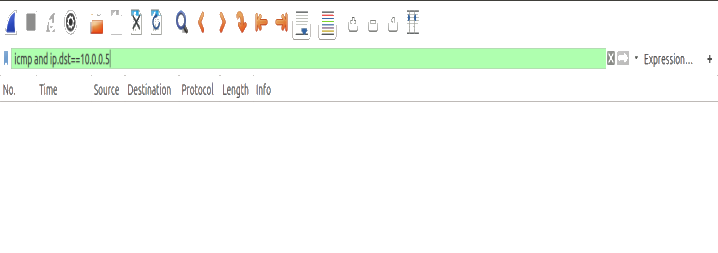
\includegraphics[scale=.6]{pics/s2-eth1-h1-ping-h5.png}
		\end{adjustbox}
	\end{figure}
	\FloatBarrier
	\begin{figure}[ht]
		\begin{adjustbox}{addcode={
			\begin{minipage}{\width}}{
				\caption{%
					Captura de wireshark monitoreando la interfaz eth1 del switch s3
					}
			\end{minipage}},rotate=360,center}
			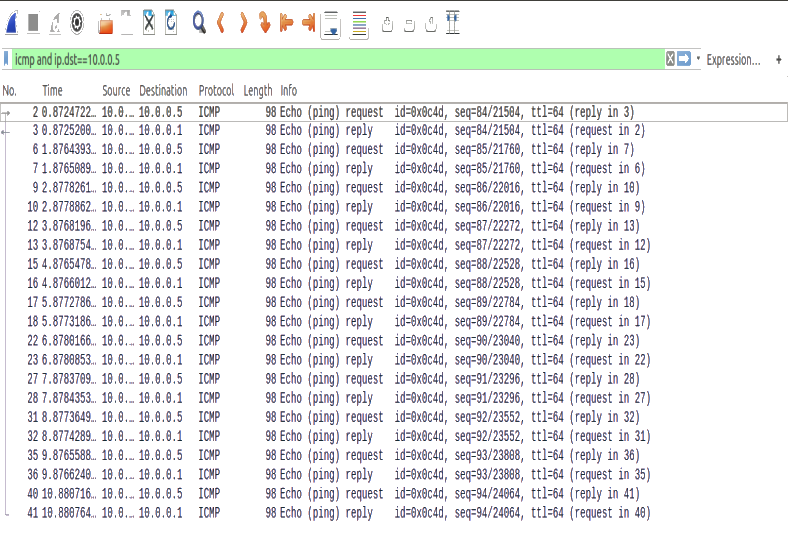
\includegraphics[scale=.6]{pics/s3-eth1-h1-ping-h5.png}
		\end{adjustbox}
	\end{figure}
	\FloatBarrier
	Luego mostramos el monitoreo en wireshark cuando hacemos el ping entre h2 y h5:\\
	\begin{figure}[ht]
		\begin{adjustbox}{addcode={
			\begin{minipage}{\width}}{
				\caption{%
					Captura de wireshark monitoreando la interfaz eth1 del switch s2
					}
			\end{minipage}},rotate=360,center}
			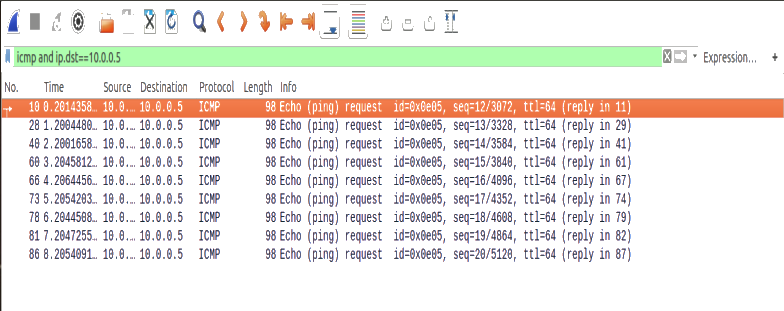
\includegraphics[scale=.6]{pics/s2-eth1-h2-ping-h5.png}
		\end{adjustbox}
	\end{figure}
	\FloatBarrier
	\begin{figure}[ht]
		\begin{adjustbox}{addcode={
			\begin{minipage}{\width}}{
				\caption{%
					Captura de wireshark monitoreando la interfaz eth1 del switch s3
					}
			\end{minipage}},rotate=360,center}
			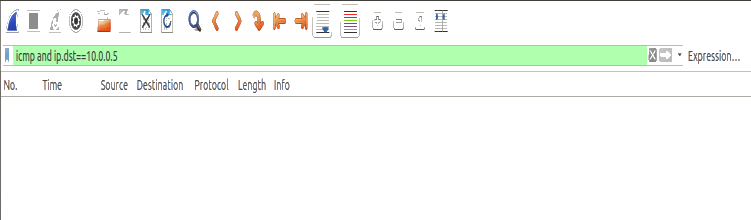
\includegraphics[scale=.6]{pics/s3-eth1-h2-ping-h5.png}
		\end{adjustbox}
	\end{figure}
	\FloatBarrier
	Como se puede observar, el ping entre h1 y h5 solo pasa por el switch 3 y el ping entre h2 y h5 solo pasa por el swtich 2.

\subsection{Denegacion de servicio}
	Para realizar esta prueba vamos a utilizar la herrmienta $iperf$ para hacer una conexxion cliente-servidor entre dos hosts. Primero, 		vamos a ir a la terminal donde esta correindo mininet (donde levatamos la topologia) y en el prompt de mininet escribiremos 
	$xterm h1 h5$ para abrir dos terminales en cada host.\\
	Luego vamos a abrir otra terminal (conectada a la VM como se exlico antes) y escribiremos: $sudo wireshark \&$. Y abriremos la interfaz 	$s5-eth1$.
	Luego en la terminal del host 5 levantaremos el servidor escribriendo lo siguiente:
	\begin{lstlisting}[language=bash,numbers=none]
		$ iperf -u -s -p 80 
	\end{lstlisting} 
	En la terminal del host 1 escribiremos lo sigueinte para hacer la conexion: 
	\begin{lstlisting}[language=bash,numbers=none]
		$ iperf -u -c 10.0.0.4 -p 80
	\end{lstlisting}
	Y lo que haremos es ver ambas ventanas de wireshark y comprobar que los paquetes TCP solo pasan por algunas de las dos interfaz, pero 		no en ambas.\\
	A continuacion mostramos la captura de las terminales en cada host y la captura de wireshark y debemos comprobar que el host 1 devuelve 	un warning el cual dice que no se pudieron enviar todos los datagramas y por lo tanto en wireshar debemos poder recibir una cantidad 		menor a la que se queria enviar.\\
	\begin{figure}[ht]
		\begin{adjustbox}{addcode={
			\begin{minipage}{\width}}{
				\caption{%
					Conexion UDP servidor host 1
					}
			\end{minipage}},rotate=360,center}
			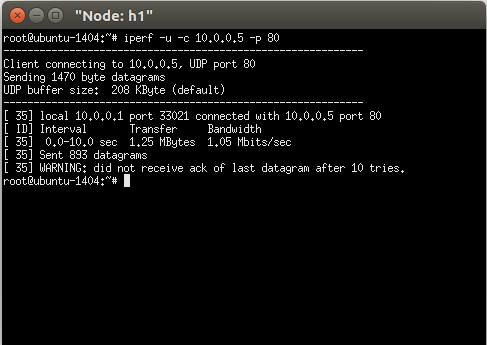
\includegraphics[scale=.6]{pics/iperf-h1-udp.png}
		\end{adjustbox}
	\end{figure}
	\FloatBarrier
	\begin{figure}[ht]
		\begin{adjustbox}{addcode={
			\begin{minipage}{\width}}{
				\caption{%
					Conexion UDP servidor host 5
					}
			\end{minipage}},rotate=360,center}
			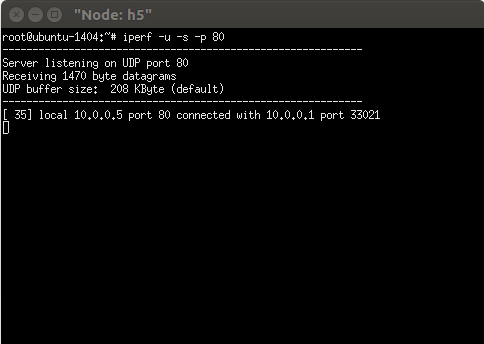
\includegraphics[scale=.6]{pics/iperf-h5-udp.png}
		\end{adjustbox}
	\end{figure}
	\FloatBarrier
	\begin{figure}[ht]
		\begin{adjustbox}{addcode={
			\begin{minipage}{\width}}{
				\caption{%
					Captura de wireshark monitoreando la interfaz eth1 del switch s5
					}
			\end{minipage}},rotate=360,center}
			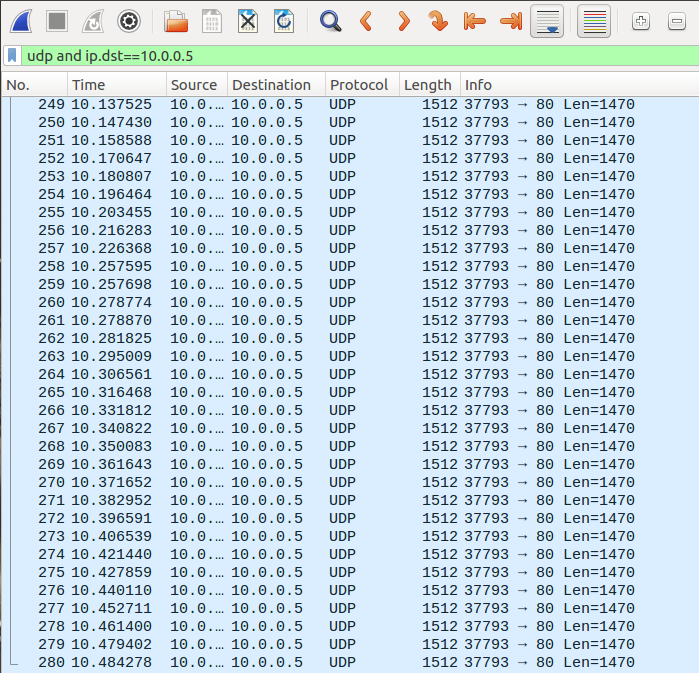
\includegraphics[scale=.6]{pics/s5-eth1-udp.png}
		\end{adjustbox}
	\end{figure}
	\FloatBarrier
	Como se puede observar, vemos que recibimos menos datagramas porque como dice en la temrinal del host 1, se quisieron enviar 893 y 		recibimos 280.
\subsection{Pruebas automaticas}
	Esta seccion se realizo a medias ya que en principio se realizaron test unitarion usando $pytest$ donde mediante wireshark, se lee la 		captura que se hizo con wireshark y se comprueba lo que se mostro anteriormente. Pero queda a modo de tareas a realizar poder ejecutar 		desde un solo script codigo que levante todas las terminales que hacen falta para podera hacer la concexion y mediante tcpdump, generar 	la capruta deseada. De esta manera, nuestros test no cambiarian, y siempre leerian un archivo $*.pcap$, donde mediante tshark se lo 		transforma en un txt para poder leerlo usando uan herramienta llamada $pandas$. En un futuro, como segundo release, se podria llevar a 		cabo dichos test y de esa manera de automatiza todo el proyecto.\\
	Para correr las pruebas, se tiene que ejecutar el siguiente comando: $sh \; scripts/test.sh$ el cual ejeuta un script que descomprime 		un archivo en la carpeta wireshark que contiene los archivos de wireshark capturados.


	\newpage
	\section{Conclusiones}

	\newpage
	\section{Anexos (Código)}
		\subsection{topology.py}
	\lstinputlisting[frame=tb, caption=Topology, label=zebra, language=Python]{../src/topology.py}
\subsection{contoller.py}	
	\lstinputlisting[frame=tb, caption=Controller, label=zebra, language=Python]{../src/controller.py}
\subsection{firewall.py}
	\lstinputlisting[frame=tb, caption=Firewall, label=zebra, language=Python]{../src/firewall.py}
\subsection{launch.py}
	\lstinputlisting[frame=tb, caption=file to launch controller and firewall, label=zebra, language=Python]{../src/launch.py}
\subsection{ecmp\_table.py}
	\lstinputlisting[frame=tb, caption=ecmp table, label=zebra, language=Python]{../src/ecmp_table.py}


	\newpage
	\section{Referencias}
		%REFERENCIAS
	\begin{enumerate}
		\item \textsc{Create a Learning Switch}\\
		\href{https://github.com/mininet/openflow-tutorial/wiki/Create-a-Learning-Switch}
		{https://github.com/mininet/openflow-tutorial/wiki/Create-a-Learning-Switch}
		\item \textsc{Open Datapath}\\
		\href{https://www.opennetworking.org/technical-communities/areas/specification/open-datapath/}
		{https://www.opennetworking.org/technical-communities/areas/specification/open-datapath/}
		\item \textsc{Pox documentation}\\
		\href{https://noxrepo.github.io/pox-doc/html/}
		{https://noxrepo.github.io/pox-doc/html/}
		\item \textsc{Visualizador de topologias}\\
		\href{http://demo.spear.narmox.com/app/?apiurl=demo#!/mininet}
		{http://demo.spear.narmox.com/app/?apiurl=demo\#!/mininet}
	\end{enumerate}

\end{document}
